\documentclass[10pt,aspectratio=169]{beamer}

% All the boilerplate is in deslides.sty
\usepackage{deslides}

\author{Ji\v{r}\'i Lebl}

\institute[OSU]{%
Oklahoma State University%
%Departemento pri Matematiko de Oklahoma {\^S}tata Universitato%
}

\title{18. Mechanical vibrations, part 2: free damped motion\\(Notes on Diffy Qs, 2.4)}

\date{}

\begin{document}

\begin{frame}
\titlepage

%\bigskip

\begin{center}
The textbook: \url{https://www.jirka.org/diffyqs/}
\end{center}
\end{frame}

\begin{frame}
\hfill\scalebox{0.85}{\subimport*{../figures}{massfigforce.pdf_t}}

\vspace*{-0.8in}

Consider 
\quad
$m x'' + c x' + kx = 0$
\quad
with $c > 0$.

(damping is present)

\medskip
\pause

Rewrite the equation as

\medskip

\qquad
$\displaystyle
x'' + 2p x' + \omega_0^2 x = 0,
\qquad
\text{where}
\qquad
\omega_0 = \sqrt{\frac{k}{m}}, \qquad p = \frac{c}{2m} .
$

\pause
\medskip

Characteristic equation:
\quad $r^2 + 2 pr + \omega_0^2 = 0$.

\pause
\medskip

Roots:
\quad $r = -p \pm \sqrt{p^2 - \omega_0^2}$.

\medskip
\pause

Solution depends on roots being real or complex, that is, if
\[
p^2 - \omega_0^2 = {\left( \frac{c}{2m} \right)}^2 - \frac{k}{m}
= \frac{c^2 - 4km}{4m^2}
\qquad
\text{is positive or negative.}
\]

\medskip
\pause

Real roots if \quad $c^2 - 4km \geq 0$ \quad or \quad $c \geq 2\sqrt{km}$ \quad
(overdamped / critically damped)

\medskip
\pause

Complex roots if \quad $c^2 - 4km < 0$ \quad or \quad $c < 2\sqrt{km}$ \quad
(underdamped)

\end{frame}

\begin{frame}
\textbf{Case 1:}
Overdamped, \quad $c^2-4km > 0$.

\medskip
\pause

Two real roots: \quad $r_1,r_2 = -p \pm \sqrt{p^2 - \omega_0^2}$.

\medskip
\pause

Both roots negative as \quad $\sqrt{p^2 - \omega_0^2} < p$.

\medskip
\pause

Solution: \quad
$x(t) = C_1 e^{r_1 t} + C_2 e^{r_2 t}$.

\vspace*{-1.1in}

\hfill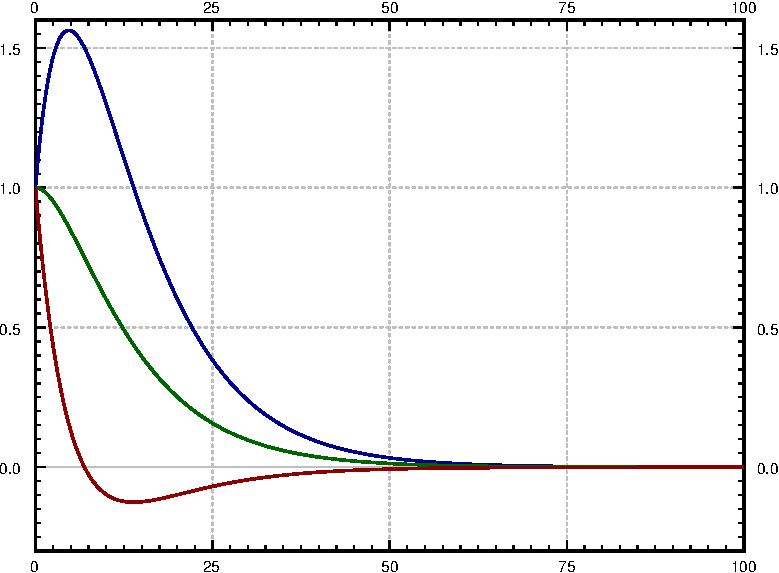
\includegraphics[width=2.5in]{../figures/mv-overdamped}

\vspace*{-0.69in}

\pause
As $r_1,r_2$ are negative, \quad
$x(t) \to 0$ as $t \to \infty$.

\medskip
\pause

No oscillation:

The graph crosses the
$t$-axis at most once.

\pause

Why?  Solve $0 = C_1 e^{r_1 t} + C_2 e^{r_2 t}$,

\pause

\thus\quad $C_1 e^{r_1 t} = - C_2 e^{r_2 t}$
\pause
\wthus
$\frac{-C_1}{C_2} = e^{(r_2-r_1) t}$
\wthus
at most one solution! (or no solution)

\medskip
\pause

\textbf{Example:}
The mass is released from rest at position $x_0$:
$x(0) = x_0$ and $x'(0) = 0$.
\[
x(t) = \frac{x_0}{r_1-r_2} \left(r_1 e^{r_2 t} - r_2 e^{r_1 t} \right) .
\]
\end{frame}

\begin{frame}
\textbf{Case 2:} 
Critically damped, \quad $c^2 - 4km = 0$.

\medskip
\pause

Only one root: \quad $-p$.

\medskip
\pause

Solution
\[
x(t) = C_1 e^{-pt} + C_2 t e^{-pt} .
\]

\medskip
\pause

Behavior very similar to overdamped: After all, infinitely close
to overdamped.

\medskip
\pause

Everything is an approximation of reality,
so best not to dwell on this edge case.

\end{frame}

\begin{frame}
\textbf{Case 3:}
Underdamped, \quad
$c^2 - 4km < 0$.

\medskip
\pause

Roots are complex:

%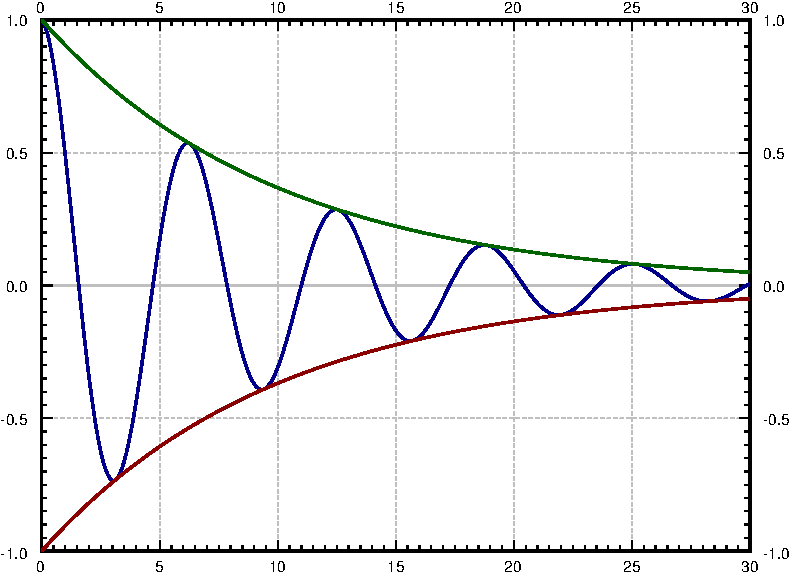
\includegraphics[width=3in]{../figures/mv-underdamped}

%Underdamped motion with the envelope curves shown.\label{mv:underdampedfig}

\quad
$
\displaystyle
r  =
-p \pm \sqrt{p^2 - \omega_0^2}
\pause
 = 
-p \pm \sqrt{-1}\sqrt{\omega_0^2 - p^2}
$

\medskip
\pause

$\quad\phantom{r}
 = 
-p \pm i \omega_1$,
\quad
where $\omega_1 =\sqrt{\omega_0^2 - p^2}$.

\medskip
\pause

Solution:

\medskip

\quad$\displaystyle
x(t) = e^{-pt} \bigl( A \cos (\omega_1 t) + B \sin (\omega_1 t) \bigr)$,
\quad or

\medskip

\quad$\displaystyle
x(t) = C e^{-pt} \cos ( \omega_1 t - \gamma )$.

\vspace*{-1.8in}

\hfill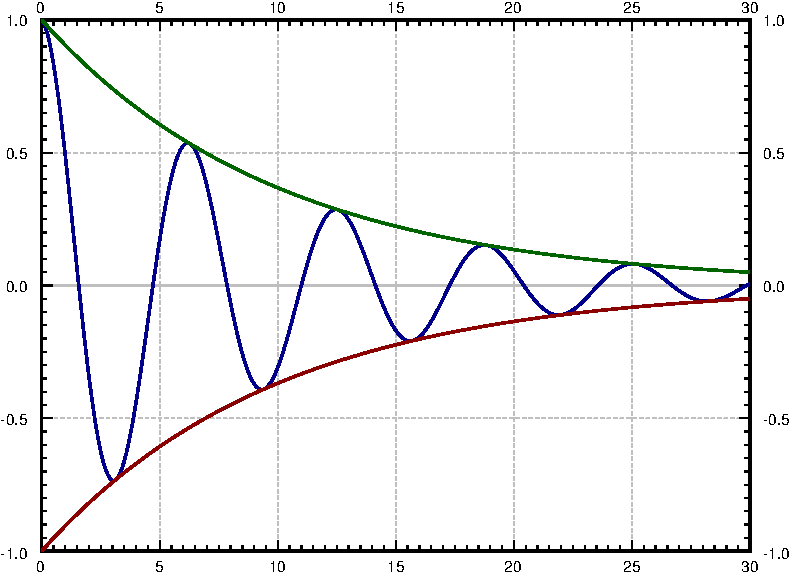
\includegraphics[width=2.5in]{../figures/mv-underdamped}

\vspace*{-0.0in}

\pause
Figure shows
\emph{envelope curves}
$C e^{-pt}$ and $-C e^{-pt}$.

\pause
Still $x(t) \to 0$ as $t \to \infty$.

\medskip
\pause

$\omega_1$ is the angular \emph{pseudo-frequency}
and is always smaller than $\omega_0$.

\medskip
\pause

$\omega_1$ gets smaller and smaller as $c$ (and hence $p$) grows.

\medskip
\pause

As $c^2$ gets close to $4km$, $\omega_1$ approaches 0.
\quad
\pause
As $c$ gets close to 0, $\omega_1$ approaches $\omega_0$.

\medskip
\pause

The envelope curves become flatter and flatter as $c$ (and hence $p$) goes to $0$.
\end{frame}


\end{document}
